\documentclass{article}
\usepackage[margin=1in]{geometry}
\usepackage{amsmath,amsthm,amssymb}
\usepackage{bbm,enumerate,mathtools}
\usepackage{tikz,pgfplots}
\usepackage{chessboard}
\usepackage[hidelinks]{hyperref}
\usepackage{multicol} % Problem 35

\newenvironment{question}{\begin{trivlist}\item[\textbf{Question.}]}{\end{trivlist}}
\newenvironment{note}{\begin{trivlist}\item[\textbf{Note.}]}{\end{trivlist}}
\newenvironment{references}{\begin{trivlist}\item[\textbf{References.}]}{\end{trivlist}}
\newenvironment{related}{\begin{trivlist}\item[\textbf{Related.}]\end{trivlist}\begin{enumerate}}{\end{enumerate}}


\begin{document}
\rating{3}{2}
Define an $n$-triangle to be a triangle with integer coordinates and perimeter
in $[n, n+1)$.
\begin{figure}[!h]
  \centering
  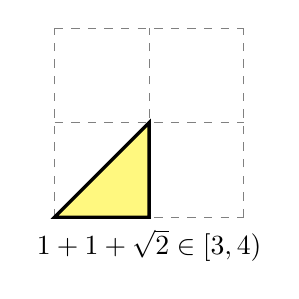
\begin{tikzpicture}[scale=1.2]
    \draw[gray, dashed] (0,0) grid (2,2);
    \draw[very thick, fill={yellow}, fill opacity=0.5] (0,0)--(1,0)--(1,1)--cycle;
    \node at (1, -0.3) {$1 + 1 + \sqrt{2} \in [3, 4)$};
  \end{tikzpicture}
  \\~\\
  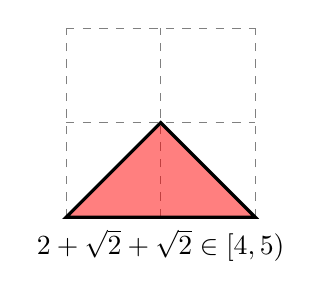
\begin{tikzpicture}[scale=1.2]
    \draw[gray, dashed] (0,0) grid (2,2);
    \draw[very thick, fill={red}, fill opacity=0.5] (0,0)--(1,1)--(2,0)--cycle;
    \node at (1, -0.3) {$2 + \sqrt{2} + \sqrt{2} \in [4, 5)$};
  \end{tikzpicture}
  ~~~
  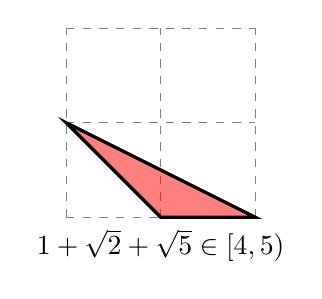
\begin{tikzpicture}[scale=1.2]
    \draw[gray, dashed] (0,0) grid (2,2);
    \draw[very thick, fill={red}, fill opacity=0.5] (1,0)--(2,0)--(0,1)--cycle;
    \node at (1, -0.3) {$1 + \sqrt{2} + \sqrt{5} \in [4, 5)$};
  \end{tikzpicture}
  \\~\\
  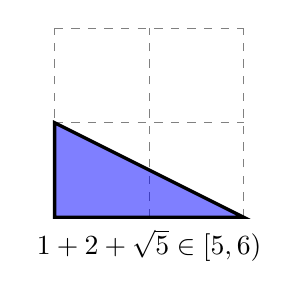
\begin{tikzpicture}[scale=1.2]
    \draw[gray, dashed] (0,0) grid (2,2);
    \draw[very thick, fill={blue}, fill opacity=0.5] (0,0)--(2,0)--(0,1)--cycle;
    \node at (1, -0.3) {$1 + 2 + \sqrt{5} \in [5, 6)$};
  \end{tikzpicture}
  ~~~
  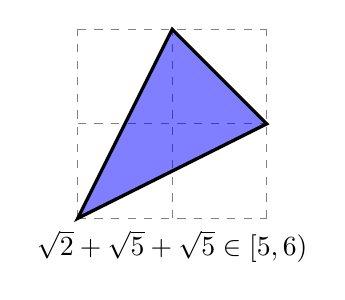
\begin{tikzpicture}[scale=1.2]
    \draw[gray, dashed] (0,0) grid (2,2);
    \draw[very thick, fill={blue}, fill opacity=0.5] (0,0)--(2,1)--(1,2)--cycle;
    \node at (1, -0.3) {$\sqrt{2} + \sqrt{5} + \sqrt{5} \in [5, 6)$};
  \end{tikzpicture}
  \caption{
    An example in yellow showing that $a(3) = 1$, and example in red showing
    that $a(4) = 2$, and an example in blue showing that $a(5) = 3$.
  }
\end{figure}
\begin{question}
  Let $a(n)$ count $n$-triangles up to dihedral action. What is the asymptotic
  growth of $a(n)$?
\end{question}
\begin{related}
  \item How many tetrahedra?
  \item How many quadrilaterals?
\end{related}
\begin{references}
  \item \url{https://oeis.org/A298079} counts the number up to congruence.
  \item Problem 44
\end{references}

\end{document}
